\documentclass[12pt,letterpaper]{article}

% just for the example
\usepackage{lipsum}
% Set margins to 1.5in
\usepackage[margin=1.5in]{geometry}

\usepackage{enumitem}

% for graphics
\usepackage{graphicx}
\graphicspath{{./figures/p3/}}

% for crimson text
\usepackage{crimson}
\usepackage[T1]{fontenc}

% setup parameter indentation
\setlength{\parindent}{0pt}
\setlength{\parskip}{6pt}

% for 1.15 spacing between text
\renewcommand{\baselinestretch}{1.15}

% For defining spacing between headers
\usepackage{titlesec}
% Level 1
\titleformat{\section}
  {\normalfont\fontsize{18}{0}\bfseries}{\thesection}{1em}{}
% Level 2
\titleformat{\subsection}
  {\normalfont\fontsize{14}{0}\bfseries}{\thesection}{1em}{}
% Level 3
\titleformat{\subsubsection}
  {\normalfont\fontsize{12}{0}\bfseries}{\thesection}{1em}{}
% Level 4
\titleformat{\paragraph}
  {\normalfont\fontsize{12}{0}\bfseries\itshape}{\theparagraph}{1em}{}
% Level 5
\titleformat{\subparagraph}
  {\normalfont\fontsize{12}{0}\itshape}{\theparagraph}{1em}{}
% Level 6
\makeatletter
\newcounter{subsubparagraph}[subparagraph]
\renewcommand\thesubsubparagraph{%
  \thesubparagraph.\@arabic\c@subsubparagraph}
\newcommand\subsubparagraph{%
  \@startsection{subsubparagraph}    % counter
    {6}                              % level
    {\parindent}                     % indent
    {12pt} % beforeskip
    {6pt}                           % afterskip
    {\normalfont\fontsize{12}{0}}}
\newcommand\l@subsubparagraph{\@dottedtocline{6}{10em}{5em}}
\newcommand{\subsubparagraphmark}[1]{}
\makeatother
\titlespacing*{\section}{0pt}{12pt}{6pt}
\titlespacing*{\subsection}{0pt}{12pt}{6pt}
\titlespacing*{\subsubsection}{0pt}{12pt}{6pt}
\titlespacing*{\paragraph}{0pt}{12pt}{6pt}
\titlespacing*{\subparagraph}{0pt}{12pt}{6pt}
\titlespacing*{\subsubparagraph}{0pt}{12pt}{6pt}

% Set caption to correct size and location
\usepackage[tableposition=top, figureposition=bottom, font=footnotesize, labelfont=bf]{caption}

% set page number location
\usepackage{fancyhdr}
\fancyhf{} % clear all header and footers
\renewcommand{\headrulewidth}{0pt} % remove the header rule
\rhead{\thepage}
\pagestyle{fancy}

% Overwrite Title
\makeatletter
\renewcommand{\maketitle}{\bgroup
   \begin{center}
   \textbf{{\fontsize{18pt}{20}\selectfont \@title}}\\
   \vspace{10pt}
   {\fontsize{12pt}{0}\selectfont \@author} 
   \end{center}
}
\makeatother

% Used for Tables and Figures
\usepackage{float}

% For using lists
\usepackage{enumitem}

% For using APA Citation format
\usepackage{apacite}

% Custom Quote
\newenvironment{myquote}[1]%
  {\list{}{\leftmargin=#1\rightmargin=#1}\item[]}%
  {\endlist}
  
% Create Abstract 
\renewenvironment{abstract}
{\vspace*{-.5in}\fontsize{12pt}{12}\begin{myquote}{.5in}
\noindent \par{\bfseries \abstractname.}}
{\medskip\noindent
\end{myquote}
}

\begin{document}

% Set Title, Author, and email
\title{Assignment P4}
\author{Snejana Shegheva \\ sshegheva3@gatech.edu}

\maketitle
\thispagestyle{fancy}

\subsection*{Question 1 - GOMS Model to Contact a Professor for Grade Explanation}

\textbf{Initial Situation}. The student has a question about their grade. The student is part of the OMSCS program that by nature of its remoteness does not provide physical access to the professor.

\textbf{Selection Rules}.

\begin{itemize}
    \itemsep0em 
    \item If the conversation needs to be formal choose method \textbf{Private Piazza Post}
    \item If the conversation is formal and urgent, choose method \textbf{Email}\footnote{This rule works under the assumption that professors more frequently check their emails than visit Piazza. Typically this rule is discussed as logistics of taking the class}
    \item If the conversation is casual \footnote{For example, the student and the professor are close friends, or the professor prefers to engage in a more social interaction}, choose method \textbf{Slack}
\end{itemize}

\textbf{Method Private Piazza Post}

\begin{itemize}
    \itemsep-0.2em 
    \item Open a web browser \footnote{The method is describing access via a web interface. The alternative via App is not considered in this model}  $\sim$ 1 sec
    \item Go to url https://piazza.com/ $\sim$ 5 sec 
    \item Log in with your Piazza credentials\footnote{The log-in step may be skipped in the certain cases where the credentials are cached} $\sim$ 5 sec 
    \item Select a class for which the grade explanation is needed $\sim$ 1 sec
    \item Select \textit{New Post} $\sim$ 1 sec
    \item Leave the \textit{Post Type} as \textit{Question} $\sim$ 1 sec
    \item Select \textit{Post to Instructors} $\sim$ 1 sec
    \item Start typing Professor's Name  $\sim$ 3 sec
    \item Select the right name from the suggested list $\sim$ 1 sec
    \item Select a folder than matches the topic, \textit{assignments} or \textit{test} $\sim$ 1 sec
    \item Enter a summary for the question, for example \textit{Grade clarification for Assignment X} $\sim$ 1 min
    \item Type the question asking for a grade explanation\footnote{The time for entering the question dependent of the scope and person's individual capabilities and preferences} $\sim$ 5 min
    \item Attach any artifacts if needed to provide an additional context $\sim$ 2 min
    \item Press \textit{Post My Question} $\sim$ 1 sec
    \item Confirm that the question has been posted by observing that it appears in the list of recent questions. $\sim$ 1 sec
\end{itemize}

\textbf{Method Email}

\begin{itemize}
    \itemsep-0.2em 
    \item Open a web browser  $\sim$ 1 sec
    \item Go to https://gmail.com/ $\sim$ 5 sec 
    \item Log in into your account \footnote{The log-in step may be skipped if the system remembers the user with any password management system} $\sim$ 5 sec 
    \item Press \textit{Compose} button. 
    \item Enter Professor's email in the \textit{To} section $\sim$ 1 sec
    \item Enter a subject identifying the class and the intent of the email\footnote{In the previous method identifying the class in the subject may not be necessary as that was selected in the higher level} $\sim$ 1 min
    \item Type the question asking for a grade explanation $\sim$ 5 min
    \item Attach any artifacts if needed to provide an additional context $\sim$ 2 min
    \item Press \textit{Send}
    \item Confirm that the email was sent by looking into the \textit{Sent} folder $\sim$ 3 sec
\end{itemize}

\textbf{Method Slack}

\begin{itemize}
    \itemsep-0.2em 
    \item Open the Slack App  $\sim$ 1 sec
    \item Go to the channel for the class $\sim$ q sec 
    \item Press + for the Direct Message
    \item Start typing the Professor's name $\sim$ 1 sec
    \item Select the professor's name $\sim$ 1 sec
    \item Press \textit{Go}
    \item Type the message $\sim$ 1 min
    \item Press \textit{Enter} $\sim$ 1 sec
\end{itemize}

\textbf{Goal}. Professor is contacted with the question for the grade explanation.

\subsection*{Question 2 - Hierarchical Task Analysis for Submitting an Assignment to Canvas}

\begin{enumerate}
    \item \textbf{Complete an assignment} <- top level task
    \begin{enumerate}
        \item \underline{Submit the assignment}
            \begin{enumerate}
                \item Find the assignment page 
                \begin{enumerate}
                    \item \textit{Go to Canvas by visiting https://gatech.instructure.com/}\footnote{The operators are presented in italic font to aid differentiation between a sub-task and an atomic operator}
                    \item \textit{Click on the class CS6750 - Human-Computer Interaction from the Canvas Dashboard}
                    \item \textit{Navigate to Assignments}
                    \item \textit{In the Upcoming Assignments section select that Assignment P4 \footnote{The assignment P4 should be listed at the top of the section}}
                    \item \textit{Click on the link Assignment P4}
                \end{enumerate}
                \item Attach the artifact
                \begin{enumerate}
                    \item \textit{Press Submit Assignment button}
                    \item \textit{Scroll to the bottom of the page}
                    \item \textit{Stay on the tab File Upload}
                    \item \textit{Press Choose File}
                    \item \textit{Browse to the correct file to your local directory}
                    \item \textit{Press Submit}
                    \item \textit{Scroll back to the top of the page}
                    \item \textit{Observe Submission information that details the status and the timestamp of the submission}
                \end{enumerate}
            \end{enumerate}
        \item \underline{Check the grade}
            \begin{enumerate}
                \item Go to Grades
                \begin{enumerate}
                    \item \textit{Go to Canvas by visiting https://gatech.instructure.com/}
                    \item \textit{Click on the class CS6750}
                    \item \textit{Navigate to Grades}
                \end{enumerate}
                \item Get the Score
                    \begin{enumerate}
                    \item \textit{Scroll-down to the Assignment P4}
                    \item \textit{Observe the grade from the Score column}
                \end{enumerate}
            \end{enumerate}
        \item \underline{Check the feedback}
            \begin{enumerate}
                \item Go to Grades (repeat task (b).i)
                \item View feedback
                    \begin{enumerate}
                        \item \textit{Scroll-down to the Assignment P4}
                        \item \textit{Click on the link Assignment P4}
                        \item \textit{Observe the text of the feedback on the right panel}
                \end{enumerate}
            \end{enumerate}
    \end{enumerate}
\end{enumerate}

\begin{itemize}
    \item Plan 0: Do (a) if the assignment has not been submitted
    \item Plan 1: Do (b) if you have received an email with keywords "Assignment Graded" in the subject
    \item Plan 2: Do (c) if you have received an email with a subject "Recent Canvas Notifications" and keywords "..just made a new comment..." in the email content. 
\end{itemize}

\subsection*{Question 3 - Distributed Cognition for Road Navigation \footnote{The answer to this question was heavily leaning to papers from ~\cite{hutchins1995cockpit} and ~\cite{nardi1996studying}}}

The couple on their voyage from start A to destination B is a part of a larger distributed cognition system. The passenger is typically designated as a person reading the map and giving the instructions to the driver. Here, the latter plays the role of \textbf{acting}, while the former is appointed to \textbf{reasoning}. Although each person in this system has their primary function, they also can be seen as performing the \textit{action} and \textit{reasoning} interchangeably. The passenger who reads the map is \textit{acting} on the map by interacting with it (flipping pages, rotating, marking routes, etc.). The driver \textit{reasons} on the car controllers and on the surrounding environment (changing the speed levels, obeying the traffic rules, reading and interpreting to road signs, etc.). 

The map itself serves as an external \textbf{memory} of the route, so the passenger who guides the driver does not need to remember the entire direction from start to destination. The whole map can be considered as a \textit{long-term} memory, while the current page (or a fold, depending on the map format) represent the \textit{short-term} memory. The map by itself is meaningless because it requires other agents, such the passenger to interpret it. The markings on the map that highlight some of the routes serve as a \textit{working memory} that helps visualize the chosen roads from the whole plan. The markings provide an additional artifact as a cognitive resource to reduce the cognitive load from the interpreter. This exemplifies the benefits of the distributed cognition where maps, signings, the couple are a part of the sizeable cognitive system. 

Looking at the map, the passenger has to orient it in the right direction to interpret the road charts correctly. This specific cognitive function can be offloaded to a compass that serves as a \textbf{perception}. Working out the answer, such as where is north or south, using the compass tool, again extends the individual's working memory. They do not need to keep track for how many times they have turned to orient themselves correctly. Other artifacts, such as road signs, can serve a similar function of helping to perceive the orientation. Additionally, the travelers can stop at the gas stations and ask for directions if the map, compass, and the street signs are insufficient for planning and executing the trip.

From the perspective of a \textbf{social cognition}, the couple may share their \textit{rememberings} and \textit{perceptions} based on the previously held conversations and experiences. The interaction here may turn out to be very complex in a sense that it can take into account the history of the relationships and their mutual awareness of each other's individuality. If the passenger is aware of the driver's nearsightedness that limits the distance from where the driver can read the signs, the passenger acts as a part of a social cognitive system by interpreting some of the signs in advance. Similarly, if the driver is aware that their partner who interpreters the map and gives the directions, tends to confuse the \textit{right} from the \textit{left} (hypothetically), then their collaborative cognition may involve confirming the direction where it mismatches their expectation based on the perception of the general direction of the trip. 

The distributed cognition without the social aspect does not place emphasis on the individualism of people involved. The collaboration is therefore viewed in the scope of information exchange between the components of the system. The enrichment comes from the social interaction where the knowledge can be shared, and the agent's actions are coordinated with a sense of a common goal. 


\subsection*{Question 4 - Distributed Cognition on the example of Yousician App}

Yousician is an innovate application with elements of game playing that allows students to learn how to play piano, guitar, and other musical instruments\cite{eli2017yousician}. It is a fun, educational app that involves following step-by-step tutorials, exercises, and play-alongs. Figure~\ref{fig::2} shows an example of a screen that user interacts with. Our obvious \textbf{task} here is \textit{playing} the provided music sheets.

\begin{figure}[h]
\centering
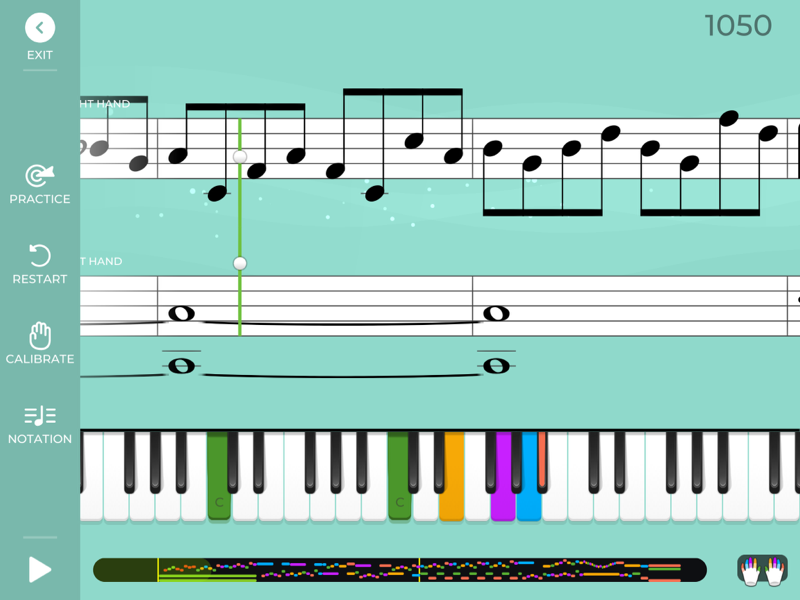
\includegraphics[scale=.35]{figures/p3/yousician.png}
\caption{A screenshot from Yousician App that teachers the user to play piano}
\label{fig::2}
\end{figure}

The shown music score serves as an external \textbf{memory} unit, as the user does not need to remember the structure of all notes. The person interacting with the interface, reads, and \textbf{reasons} over the note arrangement to play the matching notes on the piano keyboard. Here, the physical keyboard is being \textbf{acted} upon that produces a sound. Both, the person and the piano keyboard, can be seen as \textit{actors} in this cognitive system. The person presses (acts on) the key which activates a small hammer inside the piano that hits (acts on) a string or strings. 

The device through which the piano and app are connected listens to the produced pitches and \textbf{perceives} the accuracy of the play. Here again, the human also \textbf{perceives} the sounds, however his/her cognitive load for interpreting the correctness of each note is reduced by distributing the evaluation to the device (iPad, laptop, smartphone).  A user simultaneously interacts with multiple interfaces - the physical keyboard, the device with the app (microphone), the app itself which functionally includes capturing the interpreting the sound produced by the keyboard. 

Another aspect of \textbf{memory} unit is being able to re-play the entire piece so that the user can \textbf{reason} on the quality of their performance. They may not remember where they made mistakes and how many. They may not even perceive that some pitches were incorrect. Being able to review the performance after with a visual interface helps them \textit{remember} the mistakes made during the execution. By highlighting the wrong notes, the interface can be thought as a reasoning artifact. Within the distributed cognitive system, each component is considered to share a cognitive function even if the object is not animated. The critical aspect is that \textit{each} component contributes to the cognition of the system via one or several activities. There is no sharp delineation between roles and activities among the components. We have shown how one operation can be shared across portions of the system, both human and artifact alike. 

\bibliographystyle{apacite} 
\bibliography{bibtemp}

\end{document}
